\documentclass[a4paper,11pt]{article}
\usepackage[latin1]{inputenc}
\usepackage[T1]{fontenc}
\usepackage{bbm}
\usepackage{amsmath}
\usepackage{indentfirst}
\usepackage{fullpage}
\usepackage{url}
\usepackage{geometry}
\geometry{verbose,tmargin=3cm,bmargin=2cm,lmargin=2cm,rmargin=2cm}
\usepackage{graphicx}
\usepackage{epstopdf}
\usepackage[center,footnotesize]{caption}
\usepackage[section]{placeins}
\usepackage{subfig}

\DeclareRobustCommand{\greektext}{%
  \fontencoding{LGR}\selectfont\def\encodingdefault{LGR}}
\DeclareRobustCommand{\textgreek}[1]{\leavevmode{\greektext #1}}
\DeclareFontEncoding{LGR}{}{}
\DeclareTextSymbol{\~}{LGR}{126}

\title{Series 4}
\date{October 11, 2011}
\author{Genomics and bioinformatics - Week 4}

\begin{document}
\maketitle

\section{Sequence alignment}
The Needlman-Wunsch algorithm uses a method called ``dynamic programming''. This is a very general programming technique. It involves three main steps:
\begin{enumerate}
\item Initialization
\item Scoring (matrix fill)
\item Alignment (backtracking)
\end{enumerate}

In the first exercise of this session you will manually perform a global alignment of two sequences based on the following scoring scheme:

\emph{Match:} \texttt{+1}, \emph{Mismatch:} \texttt{-1}, \emph{Gap:} \texttt{-2}\\

Sequence 1: \texttt{GAATTCAGA}

Sequence 2: \texttt{GGATCGA}.

\vspace{0.5cm}

\begin{center}
\includegraphics[width=0.8\textwidth]{matrix.png}
\end{center}

Solution:\\

\section{Pair Hidden Markov Model}

In this exercise, we will construct a pair Hidden Markov Model for
the same sequences as in the first exercise and align them using the
path with maximum probability.

The maximum probability path and the corresponding alignment are calculated by a dynamic
programming algorithm which is called the Viterbi Algorithm. You will
see in the exercise that the Viterbi algorithm is actually similar
to the Needleman-Wunsch algorithm.

A general pair HMM is shown in Figure 1. It consists of the following parameters:
\begin{figure}
\begin{centering}
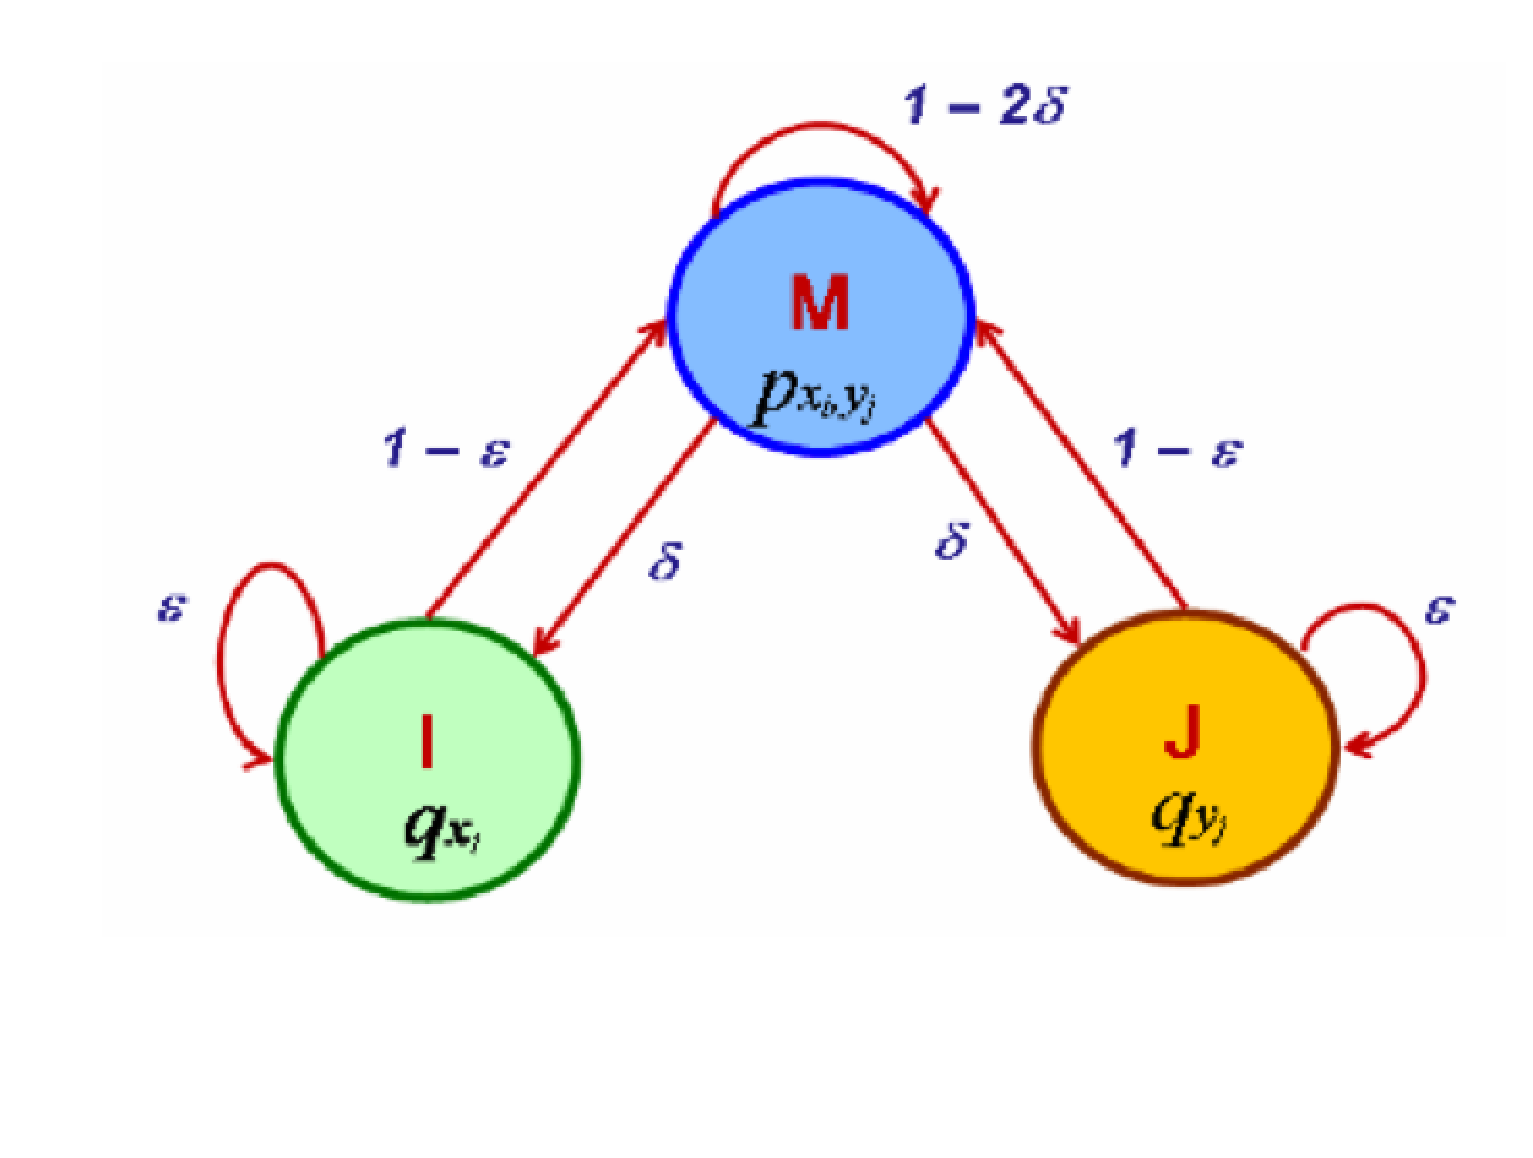
\includegraphics[width=4in]{HMMfigures.eps}\caption{Pair Hidden Markov Model}
\par\end{centering}
\end{figure}

\begin{itemize}
\item Three states: M, I, D.\\
State M matches one letter from each sequence\\
State I inserts a gap in the second sequence \\
State D inserts a gap in the first sequence

\item Emission probabilities: p(x y), q(x) and q(y), where,\\
p (x,y) = probability of emitting a pair of characters {[}x,y{]} \\
qx = probability of emitting a pair of character {[}x,\_{]}\\
qy = probability of emitting a pair of characters{[}\_,y{]}

\item Transition probabilities:\\
\textgreek{d} = probability of opening a gap \\
\textgreek{e} = probability of extending a gap \\
\end{itemize}

Find the maximum probability path, and deduce the best possible alignment.

\end{document}
